\section{Project Management}
\subsection{Agile}
Agile development is a methodology comprised of several principles and methods for project management. Where other project management methodologies such as the waterfall methodology focuses on long term rigid development, Agile takes a short term iterative approach. This provides a level of flexibility suited to a Software Development cycle, due to the unpredictable nature of inevitable setbacks such errors during the software development cycle. This helps to increase production, reduce the scope and costs of a project \cite{8078177} .

\subsection{Scrum}
A scrum is a flexible method the divides periods of work into sprints. Each sprint is a relatively short period often between 1 and 2 weeks, after which the team and stakeholders will discuss the project as a whole, reevaluate their progress from the previous sprint and plan the following one accordingly. This makes the Scrum Methodology ideally suited to work with Agile Development \cite{9136647}

\section{Tools for Project Management}

\subsection{Github}
\includegraphics[scale=0.025]{./img/Github.PNG}
 is a web-based collaborative platforms providing tools to ease distributed development \cite{7887704}. Officially launched in 2008, it uses Git a decentralized version control system that hosts code and using a master-less peer-to-peer replication to allow relatively seamless collaboration between developers on the same project.

\subsection{Microsoft Teams}

\includegraphics[scale=0.025]{./img/Teams.jpg}
Microsoft Teams is a chat-based collaboration platform, that allows for document sharing, online meeting other useful tools for communication.  Teams allows for collaboration between members whether it be through the messaging platform or voice and video calls \cite{teams}.

\subsection{Discord}

\includegraphics[scale=0.025]{./img/Discord.PNG}
Discord is a free voice communications app used for voice chat, video and messaging between friends. Discord can be used for simple communication but has the facilities to allow for a more professional type of communication.  These facilities include group and one-to-one private messaging in which members can text, voice and video chat. Discord provides facilities sharing of documentation, useful links and one's screen which allows for real time sharing of information proving to be invaluable towards the development of a project \cite{discord}.

\section{Application Development Tools}
\subsection{Visual Studio Code}

\includegraphics[scale=0.025]{./img/VsCode.PNG}
Visual Studio Code is a lightweight source code editor created by Microsoft. It has many plugins that can easily be added called extensions that allow the user to customize and add shortcuts to their project based on what language they would like to use as well as allowing the creation of community made extensions. It has built in support for Azure, Github and IntelliSense \cite{vscode}.

\section{Front End}
\subsection{Angular JS}

\includegraphics[scale=0.025]{./img/Angular.PNG}
Angular is a widely used web development framework that creates a single page client application utilizing JavaScript and the Node Package Manage. It supports the editing and managing of various languages such as HTML, CSS and TypeScript while removing some of the complexities by adding specific angular attributes that would not normally be in these languages as well as easily managing a projects imports through the NPM.
\\\\
With regular updates still being made to date, it is a platform that is currently in use in a wide range of applications. An advantage of using a single-page client application was that they are commonly used and offer a wide range of possibilities and flexibility with regards to web and agile development.  With these characteristic, Angular is a platform that will mostly likely still be relevant and used for the foreseeable future and thus a valuable asset worth understanding.

\section{Back End}
\subsection{Database}

\includegraphics[scale=0.15]{./img/Firebase.jpg}
A database, in its most basic concept is a collection of information that has been organized in a way, so that it can be accessed,read, managed, updated and stored. The database used in this project this project stores a users information by creating a document with the users information entered at registration and adding that document to the 'Users' collection at the root of the database. The database is configured in a way that only gives certain permissions to users who are logged in and only allowing the user to manipulate their own data.\\\\
Relational Database Management Systems (RDMS) is the most common way of storing structure data for web applications.  The data-stores in this type of database requiring SQL, a language that provides consistent set of facilities for querying, manipulating and controlling data \cite{strauch2011nosql}. For use in this project we decided on using a NoSQl database instead as it was something unfamiliar to us.

\subsubsection{NoSQL}
In more recent years the idea of a "one size fits all" with relation to data-stores has become more popular. This has lead to the creation of alternative types of databases.  These are commonly referred to as NoSQL databases which allow for a more flexible way of storing and retrieving data then the reliable and rigid relational SQL, allowing for a wider variety of ways for structuring data which can be more easily reworked during development.  The ability to remove the complexity of a relational database and store/process data as it appears is one of NoSQL's greatest strengths in comparison to a SQL database. \\\\
The use of NoSQL can avoid unnecessary complexity and strict data consistency for applications where this might not be necessary.  NoSQL databases also allows for high throughput and horizontal scalability which is necessary when dealing with large amounts of data \cite{strauch2011nosql}. Though because of this freedom a disorganized database can be created if the developer is not careful.

\subsubsection{Firebase}
The Database we used for this project is Firebase's Cloud Firestore database. This was used for storing user information, such as messages, forum posts, friends lists and user created characters. It was selected during our research because of it's NoSQL schema and it's relatively low maintenance costs for a service of it's quality being made by Google. Firebase is the collection of Google's many services on the cloud and can be used to enhance web applications and utilize other features such as Firebase storing and Firebase Hosting. \\\\
Firestore provides methods that can be implemented into your project such as Authentication, file storage, hosting and real-time databases. A big advantage of Firebase was libraries such as AngularFireStore which provides features and methods to an angular application making them very complimentary to each other. Firebase met the projects needs as we would not have too much traffic and being limited to a certain amount did not impact the project negatively. \cite{firebase}

\subsubsection{Cloud Firestore}
Cloud Firestore is an NoSQL type database that is hosted on Google Cloud.

\subsubsection{Backend as a Service (BaaS)}
Baas is a cloud computing service model that allows developers a way of connecting web application to the cloud service using application programming languages (API) and software development kits (SDK's).

\subsection{Cloud}

\includegraphics[scale=0.15]{./img/Azure.PNG}
Many company's today provide a cooperative server-side on demand service for running online applications.  The rational behind this is that large companies have numerous large storage facilities,with often more servers then what they intend to use. By renting out some of this servers to smaller scale users, whether it be for personal of business use, allows them to reduce some of their expenses.  This allows smaller users to host applications to a world wide userbase around the world without having to deal with the expense and time costs of setting up personal servers.\\\\
The provider for the cloud computing platform used in this project is Microsoft Azure.  The use of this platform in this project is to host a virtual machine in which the project is deployed. There are several reasons behind this, first is that the users of the application would not be as badly affected by latency due to the location of the local device.  Secondly if the application was stored locally, if the device that hosts the application fails then the application would be offline. By having this on professionally maintained servers the likelihood and impact of this is greatly reduced. Finally if the application was to be expanded then it would only need to expand the server usage on Azure.

\subsubsection{The Cloud OS(Operating System)}
For a lot of cloud-computing applications the entirety of the user interface resides in a single window on the browser or by using the cloud-computing paradigm, it has the ability to host the full facilities of an operating system on a browser.  An alternative solution to this is to bypass the web browser on the local machine altogether by substituting it with a software system that runs an application on a client side computer that communicates directly with the servers on the cloud - Virtual Machine \cite{hayes2008cloud}.


\subsubsection{Azure}
Azure Cloud Deployment is Microsoft's cloud platform which is a foundation for running applications and storing data on the cloud.  Azure provides over 200 products to help build run and manage applications across the cloud with the developer being able to choose the tools and framework needed \cite{azure}.  On Azure developers can use different types of roles, in our case we are using the Virtual Machine role running a Ubuntu Server image running a single desktop \cite{chappell2009introducing}.

\subsubsection{Linux}
Linux is Operating System and is one of the most popular platforms on the planet, with it being a popular OS for computers and is the bases for Android.  An Operating System is a software that manages the use of all the hardware resources associated with any device.  The Linux OS is comprised of several different parts: bootloader, kernel, init system, daemons, graphics server, desktop environment and applications \cite{linux}.

\subsubsection{Ubuntu}

\includegraphics[scale=0.025]{./img/Ubuntu.jpg}
The OS we are using on Azure is Ubuntu, it is a complete Linux operating system that is freely available. Ubuntu is the world's most widely accessible and used Linux platform, with a Ubuntu Server being the reference OS for the OpenStack project, popular on cloud platforms such as Azure, AWS and Google Cloud \cite{ubuntu}.

\subsection{SDK's and Libraries}
\subsubsection{AngularFire}

\includegraphics[scale=0.25]{./img/AngularFire.PNG}
The AngularFire library is part of Firebase Open Source, a platform were user libraries are used and created by the firebase community. It contains predefined methods configured to make communicating with the server an easier process \cite{angularfire}.
\subsubsection{Node Package Manage}

\includegraphics[scale=0.05]{./img/NPM.PNG}
The Node package Manager was used to install/import packages and imports into the Angular project. It uses Node.js and store the packages in package.json.

\subsection{Containers}
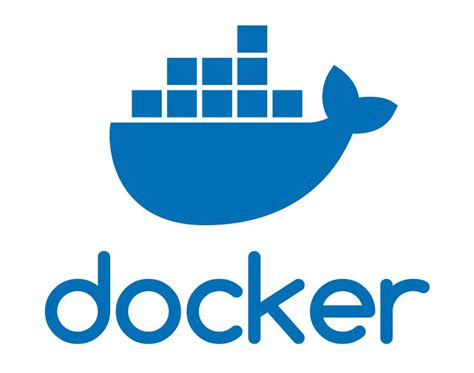
\includegraphics[scale=0.155]{./img/Docker.jpg}
A container is a software used to package up all the code and dependencies of an application so that it can be reliably and easily moved from one computer environment to another.  This can be done whether the new environment is similar to previous or completely different.  Isolating the software from the environment, is done by the use of container image which become containers at runtime \cite{container}. In this case the use of containers was used when changing from the test environment on our local computer to the production environment on the virtual machine.

\subsection{Docker}
The container software used in this project is Docker.  Docker, like any containerizing software takes away repetitive configuration throughout the development of an application and allows for easy, portable application development whether it be on desktop or cloud platform \cite{docker}.   \\\\
A Docker container image is a lightweight, standalone executable that include everything that application requires to run: setting, system libraries, code, system tools and runtime.  Images become containers when run by the docker engine, which is available on both Linux and Windows, by using the Windows Subsystem for Linux (WSL).  Docker's containerized software will always run the same, regardless of the systems infrastructure.  \\\\
An easy way to work with Docker containers is through the Docker Command Line Interface (CLI), which by use of commands simplifies how to manage the container instances.  There are three types of Docker containers that run on the Docker Engine: standard, lightweight and secure. Standard was implemented for the use of this project as it is the industry standard \cite{container}.

\subsection{Typescript}

\includegraphics[scale=0.015]{./img/TS.PNG}
Typescript is an open source language developed and maintained by Microsoft, that continues to build on JavaScript and adds optional static typing to the language. As Typescript is compiled it is converted to the specified version of JavaScript, this results in existing JavaScript programs being valid TypeScript programs.  It makes JavaScript more readable by assigning types to and definitions to variables and methods. This makes debugging a much easier process as often a problem with JavaScript is the lack of information when it cannot compile. \\\\
A big advantage of Typescript is that native JavaScript code will also work as intended as the typescript interprets the code and converts it into JavaScript during the compile process. As JavaScript is widely used in web development as it is found in some form or another on a vast amount of websites. This means that Typescript gives the flexibility of JavaScript while making it easier on the developer.

\subsubsection{Node.Js}

\includegraphics[scale=0.025]{./img/node.png}
Node is a package manager that manages and installs packages onto your machine. It is widely known and is needed to install Angular using the Node Package Manager. Much like Git is required for Github, Node is required to use NPM. NPM stores it's packages in JSON files such as package.json which Angular uses to manage a projects dependencies.


\subsection{Cmder}

\includegraphics[scale=0.155]{./img/Cmder.PNG}
Cmder is a package created as Command Line Interface that allows the user to use commands from both the Unix systems found in Linux and the console commands found in Windows. Having the same commands available of both Operating System is a big advantage as it saves time looking up the syntax.


\subsection{Testing Tools}
\subsubsection{Selinium}

\includegraphics[scale=0.015]{./img/Testing.PNG}
Selinium was used to test the feature of the web application.

\subsection{Code Examples}




